
\documentclass[ review  , 3p ]{elsarticle}
%default = preprint (single sapce), review = doublespace
%detail class option: https://www.elsevier.com/__data/assets/pdf_file/0008/56843/elsdoc-1.pdf

% eliminate "Preprinted to Elsevier"
\makeatletter
\def\ps@pprintTitle{%
 \let\@oddhead\@empty
 \let\@evenhead\@empty
 \def\@oddfoot{\centerline{\thepage}}%
 \let\@evenfoot\@oddfoot}
\makeatother

%%% Begin My package additions %%%%%%%%%%%%%%%%%%%
\usepackage[hyphens]{url}



\usepackage{lineno} % add
\providecommand{\tightlist}{%
  \setlength{\itemsep}{0pt}\setlength{\parskip}{0pt}}

\usepackage{graphicx}

\usepackage{zxjatype}
\usepackage{xeCJK}
\setCJKmainfont{ipaexm.ttf}
\setCJKsansfont{ipaexg.ttf}
\setCJKmonofont{ipaexg.ttf}

\usepackage{color}

\usepackage{booktabs}
\usepackage{longtable}
\usepackage{array}
\usepackage{multirow}
\usepackage{wrapfig}
\usepackage{float}
\usepackage{colortbl}
\usepackage{pdflscape}
\usepackage{tabu}
\usepackage{threeparttable}
\usepackage{threeparttablex}
\usepackage[normalem]{ulem}
\usepackage{makecell}
\usepackage{xcolor}


%\usepackage{xpatch}
%\xpatchcmd{\MaketitleBox}{\hrule}{}{}{}% remove first horizontal rule (above abstract)
%\xpatchcmd{\MaketitleBox}{\hrule}{}{}{}% remoce second horizonral rule (below keywords)
%%%%%%%%%%%%%%%% end my additions to header

\usepackage[T1]{fontenc}
\usepackage{lmodern}
\usepackage{amssymb,amsmath}
\usepackage{ifxetex,ifluatex}
\usepackage{fixltx2e} % provides \textsubscript
% use upquote if available, for straight quotes in verbatim environments
\IfFileExists{upquote.sty}{\usepackage{upquote}}{}
\ifnum 0\ifxetex 1\fi\ifluatex 1\fi=0 % if pdftex
  \usepackage[utf8]{inputenc}
\else % if luatex or xelatex
  \usepackage{fontspec}
  \ifxetex
    \usepackage{xltxtra,xunicode}
  \fi
  \defaultfontfeatures{Mapping=tex-text,Scale=MatchLowercase}
  \newcommand{\euro}{€}
\fi
% use microtype if available
\IfFileExists{microtype.sty}{\usepackage{microtype}}{}
\bibliographystyle{elsarticle-harvard}
\usepackage{tabularx}
\ifxetex
  \usepackage[setpagesize=false, % page size defined by xetex
              unicode=false, % unicode breaks when used with xetex
              xetex]{hyperref}
\else
  \usepackage[unicode=true]{hyperref}
\fi
\hypersetup{breaklinks=true,
            bookmarks=true,
            pdfauthor={},
            pdftitle={Short Paper},
            colorlinks=false,
            urlcolor=blue,
            linkcolor=magenta,
            pdfborder={0 0 0}}
\urlstyle{same}  % don't use monospace font for urls

\setcounter{secnumdepth}{5}

\newlength{\cslhangindent}
\setlength{\cslhangindent}{1.5em}
\newlength{\csllabelwidth}
\setlength{\csllabelwidth}{3em}
\newenvironment{CSLReferences}[3] % #1 hanging-ident, #2 entry spacing
 {% don't indent paragraphs
  \setlength{\parindent}{0pt}
  % turn on hanging indent if param 1 is 1
  \ifodd #1 \everypar{\setlength{\hangindent}{\cslhangindent}}\ignorespaces\fi
  % set entry spacing
  \ifnum #2 > 0
  \setlength{\parskip}{#2\baselineskip}
  \fi
 }%
 {}
\usepackage{calc} % for \widthof, \maxof
\newcommand{\CSLBlock}[1]{#1\hfill\break}
\newcommand{\CSLLeftMargin}[1]{\parbox[t]{\maxof{\widthof{#1}}{\csllabelwidth}}{#1}}
\newcommand{\CSLRightInline}[1]{\parbox[t]{\linewidth}{#1}}
\newcommand{\CSLIndent}[1]{\hspace{\cslhangindent}#1}

% Pandoc toggle for numbering sections (defaults to be off)


% Pandoc header


\begin{document}
  \begin{frontmatter}

    \title{Charitable Giving, Tax Reform, and Government Efficiency\tnoteref{1}}
            \tnotetext[1]{This research is base on}
                \author[Osaka University]{
      Hiroki Kato 
       \corref{*} }
     \ead{vge008kh@stundent.econ.osaka-u.ac.jp}   %to avoid auto-link, use \@ instead of @
        \author[Chiba University]{
      Tsuyoshi Goto 
      }
      %to avoid auto-link, use \@ instead of @
        \author[Kobe University]{
      Yong-Rok Kim 
      }
      %to avoid auto-link, use \@ instead of @
            \address[Osaka University]{Graduate School of Economics, Osaka University, Japan}
        \address[Chiba University]{Graduate School of Economics, Chiba University, Japan}
        \address[Kobe University]{Graduate School of Economics, Kobe University, Japan}
            \cortext[*]{Corresponding Author.}
      
        \begin{abstract}
      Brah
    \end{abstract}
      
        \begin{keyword}
      Charitable giving, Giving price, Tax reform, Governement efficiency, South Korea
       \JEL{D91, I10, I18} 
    \end{keyword}
    
  \end{frontmatter}

  \hypertarget{introduction}{%
  \section{Introduction}\label{introduction}}
  
  In many countries, governments set a tax relief for charitable giving. This is because, if subsidizing charitable giving induces a large increase in donations, it is desirable for public good provision. To evaluate the effect of tax relief, many papers investigate the elasticity of charitable donations with respect to their tax price (Almunia et al., 2020; Auten et al., 2002; Bakija and Heim, 2011; Fack and Landais, 2010; Randolph, n.d.). Focusing on the tax deduction or tax credit on the charity, they show that the price elasticity of giving is about -1 or more in terms of absolute value, which means that the tax relief for the charitable giving is good in the sense that 1\% tax relief derives more than 1\% donation.
  
  However, if the government can provide public good more efficiently than the direct donation, the donation may not be preferable because the public good provision via donation would be costly then.
  Moreover, when the government is much more efficient than charities, people may not donate so much even if they have a warm-glow preference. Saez (2004) suggests that the change of the relative price between public good provision by donation and government will change the behavior of people and the price elasticity of donation.
  However, the evaluation about the efficiency of the government is usually subjective and different for people. If someone regard the government as efficient, the perceived relative price of giving would be high for them. Thus, the giving behavior would be affected by the subjective perception towards the government.
  
  Considering these points, this paper investigates (1) the price elasticity of giving and (2) whether the different perception towards the government cause the different giving behavior using South Korean panel data.
  Our first main concern is the price elasticity of charity. South Korea (Korea hereafter) experienced the tax reform in 2014, from when the tax relief on charitable giving was conducted by tax credit, though tax deduction had been used before 2014. Thus, we exploit this tax reform as an exogenous policy change to derive the price elasticity of giving. Since the extant research focus on the tax reform within the scheme of tax deduction or tax credit, this paper firstly deals with the tax reform from tax deduction system to tax credit system.
  Our result classifies that the price elasticity of giving in Korea is -1.07 \textasciitilde{} -1.26, which is within the range of the extant research.
  
  Our second concern is the relationship between the giving behavior and the perception towards the government. As we explained, people feeling administrative inefficiency would consider the direct donation is more efficient and would have more willingness to donate. Using the Korean field data, we investigate this and show that the amount of donation is not different between those who regard government as inefficient and the others, though the giving price elasticity of the former is more elastic than the latter. This means that those who think of government as inefficient have more willingness to donate for 1\% reduction of giving price.
  
  This paper contributes two strands of charitable giving literature: the elasticity of charitable donations with respect to their tax price and the perception of government's inefficiency. The examples of papers in the first strand are Randolph (n.d.), Auten et al. (2002), Fack and Landais (2010), Bakija and Heim (2011), and Almunia et al. (2020). They typically use the tax return data, the main part of which is the data about wealthy people. Since our data is based on survey, which reflects the income distribution of population, we believe that we can estimate the giving price elasticity of population more precisely. Using the data with low-income households may be difficult to estimate the giving price elasticity in terms of intensive margin since they are expected to donate less than high-income households. To address this issue, we estimate not only the elasticity of intensive margin, as most of papers do, but also the elasticity of extensive margin following Almunia et al. (2020).
  Moreover, we use the data of Korea, a non-Western country, which the extant research did not examine\footnote{This point may be important since Kim (2021) reports that the giving behavior is strongly affected by the cultural matter such as the religious belief.}.
  
  In the second strand, there are some experimental studies and papers considering the tax evasion. Using an experiment, Li et al. (2011) compare people's willingness to give money for private charities and government agencies whose missions are the same. They show that people tend to donate for private charities more than government agency though they do not directly investigate the relationship between people's perception toward the government and giving behavior. Sheremeta and Uler (2020) show that people increase the voluntary public good provision when they face the wasteful government spending in the experimental setting. Although the government in their setting does not provide public good, they suggest that the willingness for donation may increase if people perceive the inefficiency of government. In the tax evasion literature, several paper suggests the perceived inefficiency of government reduce tax morale (Anderson, 2017; Frey and Torgler, 2007; Hammar et al., 2009). We contribute on this literature by showing the relation between the perception of government efficiency and the giving behavior.
  
  This paper consist of XXX sections. Section 2 and 3 respectively explain the institutional background and data. Section 4 deals with the analysis of giving price elasticity and section 5 shows the analysis of perceptions toward the government. We discuss the result in section 6 and section 7 concludes.
  
  \hypertarget{institutional-background}{%
  \section{Institutional background}\label{institutional-background}}
  
  In this section, we describe the income tax relief for charitable giving in Korea and used dataset.
  
  \hypertarget{tax-relief-for-charitable-giving-by-tax-deduction-and-tax-credit}{%
  \subsection{Tax relief for charitable giving by tax deduction and tax credit}\label{tax-relief-for-charitable-giving-by-tax-deduction-and-tax-credit}}
  
  In the South Korea, the tax policy about charitable giving drastically changed in 2014. Before then, tax relief of charitable giving was provided by tax deduction while, from 2014, tax relief by tax credit was introduced instead of tax deduction.
  
  The tax deduction and tax credit may have different effects on giving behavior. This subsection summarize the difference of tax deduction and tax credit.
  Consider that a household has a choice between private consumptions (\(x_i\)) and charitable giving (\(g_i\)). Let \(y_i\) be pre-tax total income.
  Then, the budget constraint is
  
  \[
      x_i + g_i = y_i - T_i(y_i, g_i).
  \]
  \(T_i\) is tax amount which depends on the pre-tax income and charitable giving.
  On one hand, tax deduction reduces taxable income by giving, that is,
  
  \[
      T_i = \tau(y_i - g_i) \cdot (y_i - g_i),
  \]
  
  where \(\tau(\cdot)\) is the marginal income tax rate which is determined by \(y_i - g_i\). The budget constraint will be
  
  \[
      x_i + [1 - \tau(y_i - g_i)]g_i = [1 - \tau(y_i - g_i)] y_i.
  \]
  
  Thus, the giving price compared to the price of private consumption is \(p_i^{d} \equiv 1 - \tau(y_i - g_i)\) in tax deduction system. Since the giving price in tax deduction scheme varies depending on (1) the income level and (2) the amount of charitable giving, it is endogenous to them, i.e. (1) and (2).
  
  On the other hand, tax credit reduces tax amount directly, that is,
  
  \[
      T_i = \tau(y_i)\cdot y_i - m g_i,
  \]
  
  where \(m \in [0, 1]\) is the tax credit rate. Under the tax credit system, the budget constraint is
  
  \[
      x_i + (1 - m) g_i = [1 - \tau(y_i)] y_i.
  \]
  
  Thus, the giving price of tax credit system will be \(p_i^c = 1 - m\), which is only dependent on the tax credit rate \(m\), which is exogenously determined by the government.
  Therefore, the giving price in the tax credit system would not be manipulated by donors.
  ---\textgreater{}
  
  \hypertarget{korean-tax-reform-in-2014-need-modification-by-kim-san}{%
  \subsection{Korean tax reform in 2014 (Need modification by Kim san)}\label{korean-tax-reform-in-2014-need-modification-by-kim-san}}
  
  The tax incentives for charitable giving in Korea stared in 2000 and the market of charitable giving in Korea totaled 10.9 trillion KRW (approximately 1.09 bilion USD, 0.761\% of GDP) in 2012 according to the national tax statistics.
  Since the income tax deduction was initially used as a tax incentive and the marginal income tax rate was determined as Table \ref{tab:tabTaxRate}, the minimum giving price before 2014 was 0.62.
  
  \begin{table}
  
  \caption{\label{tab:tabTaxRate}Marginal Income Tax Rate}
  \centering
  \fontsize{7}{9}\selectfont
  \begin{threeparttable}
  \begin{tabular}[t]{lccccccc}
  \toprule
  Income/Year & 2008 & 2009 & 2010 \textasciitilde{} 2011 & 2012 \textasciitilde{} 2013 & 2014 \textasciitilde{} 2016 & 2017 & 2018\\
  \midrule
  (A) \textasciitilde{} 1200 & 8\% & 6\% & 6\% & 6\% & 6\% & 6\% & 6\%\\
  \cmidrule{1-8}
  (B) 1200 \textasciitilde{} 4600 & 17\% & 16\% & 15\% & 15\% & 15\% & 15\% & 15\%\\
  \cmidrule{1-8}
  (C) 4600 \textasciitilde{} 8800 & 26\% & 25\% & 24\% &  & 24\% & 24\% & 24\%\\
  \cmidrule{1-4}
  \cmidrule{6-8}
  (D) 8800 \textasciitilde{} 15000 &  &  &  & \multirow{-2}{*}{\centering\arraybackslash 24\%} & 35\% &  & 35\%\\
  \cmidrule{1-1}
  \cmidrule{5-6}
  \cmidrule{8-8}
  (E) 15000 \textasciitilde{} 30000 &  &  &  & 35\% &  & \multirow{-2}{*}{\centering\arraybackslash 35\%} & 38\%\\
  \cmidrule{1-1}
  \cmidrule{5-5}
  \cmidrule{7-8}
  (F) 30000 \textasciitilde{} 50000 &  &  &  &  &  & 38\% & 40\%\\
  \cmidrule{1-1}
  \cmidrule{7-8}
  (G) 50000 \textasciitilde{} & \multirow{-4}{*}{\centering\arraybackslash 35\%} & \multirow{-4}{*}{\centering\arraybackslash 35\%} & \multirow{-4}{*}{\centering\arraybackslash 35\%} & \multirow{-2}{*}{\centering\arraybackslash 38\%} & \multirow{-3}{*}{\centering\arraybackslash 38\%} & 40\% & 42\%\\
  \bottomrule
  \end{tabular}
  \begin{tablenotes}
  \item Notes: Marginal income tax rates applied from 2008 to 2018 are summarized. The income level is shown in terms of 10,000 KRW, which is approximately 10 United States dollars (USD) at an exchange rate of 1,000 KRW to one USD.
  \end{tablenotes}
  \end{threeparttable}
  \end{table}
  
  In 2014, aiming at the relaxation of regressivity of giving price, the Korean government reformed tax system again, where the tax credit was introduced instead of tax deduction. Since then, 15\% of the total amount of charitable giving has been allowed as a tax credit, which means that the giving price from 2014 is 0.85 irrelevant to the income level.
  
  Summarizing this, compared to tax credit system, the high income household, whose (average) income tax rate is more than 15\%, get benefit from charitable giving under the tax deduction system. However, middle or low income households would enjoy tax relief in tax credit system more than tax deduction system. We exploit this policy change as an identification strategy.
  
  \hypertarget{data}{%
  \section{Data}\label{data}}
  
  \hypertarget{national-survey-of-tax-and-benefit-nastab}{%
  \subsection{National Survey of Tax and Benefit (NaSTaB)}\label{national-survey-of-tax-and-benefit-nastab}}
  
  In this paper, we use panel data from the National Survey of Tax and Benefit (NasTaB).
  NasTaB survey is an annual financial panel survey implemented by The Korea Institute of Taxation and Finance implements to study the tax burden of households and the benefits that households receive from government. The subjects of this survey are general household and household members living in 15 cities and provinces nationwide. This survey is based on a face-to-face interview. If it is difficult for investigators to meet subjects, another family member answers on behalf of him.
  
  In the analysis, we use data from 2012 to 2018 since \color{red}we focus on the 2014 tax reform.
  \color{black}In addition, we exclude the subject of the sample, whose age is under 23, since they are not likely to have income or asset.
  
  Figure \ref{fig:figDonationRate} shows the proportion of donors and the average amount of donation by donors in the NasTaB data. It shows that about 20\% of respondents in NasTaB data donate in each year and their amount of donation is about 1.7 million KRW.
  
  \hypertarget{time-series-of-chariable-giving}{%
  \subsection{Time Series of Chariable Giving}\label{time-series-of-chariable-giving}}
  
  \begin{figure}
  
  {\centering 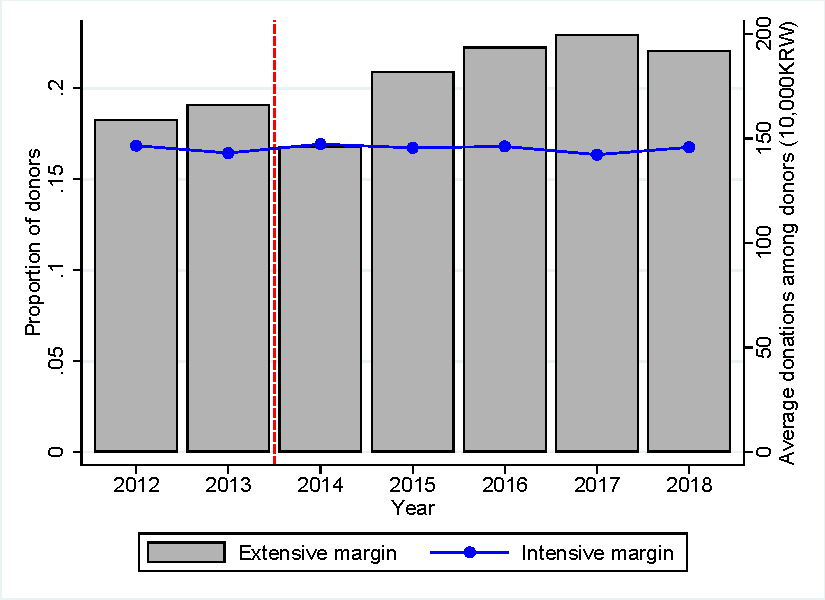
\includegraphics[width=0.9\linewidth]{C:/Users/vge00/Desktop/NaSTaB/_assets/SummaryOutcome} 
  
  }
  
  \caption{Proportion of Donors and Average Donations among Donors}\label{fig:figDonationRate}
  \end{figure}
  
  \begin{table}
  
  \caption{\label{tab:kableSummaryCovariateSlides}Summary Statistics}
  \centering
  \fontsize{7}{9}\selectfont
  \begin{tabular}[t]{lccc}
  \toprule
   & N & Mean & Std.Dev.\\
  \midrule
  \addlinespace[0.3em]
  \multicolumn{4}{l}{\textbf{Income and Giving Price}}\\
  \hspace{1em}Annual taxable income (unit: 10,000KRW) & 53269 & 1876.121 & 2700.965\\
  \hspace{1em}Giving Price & 62878 & 0.858 & 0.036\\
  \addlinespace[0.3em]
  \multicolumn{4}{l}{\textbf{Charitable Donations}}\\
  \hspace{1em}Annual charitable giving (unit: 10,000KRW) & 67849 & 29.522 & 132.914\\
  \hspace{1em}dummy of Donation > 0 & 67849 & 0.203 & 0.402\\
  \addlinespace[0.3em]
  \multicolumn{4}{l}{\textbf{Government Efficiency}}\\
  \hspace{1em}Current Tax-Welfare Balance & 29272 & -0.137 & 0.889\\
  \hspace{1em}Ideal Tax-Welfare Balance & 29273 & 0.541 & 0.721\\
  \addlinespace[0.3em]
  \multicolumn{4}{l}{\textbf{Individual Characteristics}}\\
  \hspace{1em}Age & 67848 & 51.348 & 15.806\\
  \hspace{1em}Female dummy & 67848 & 0.525 & 0.499\\
  \hspace{1em}University graduate & 67842 & 0.411 & 0.492\\
  \hspace{1em}High school graduate & 67842 & 0.350 & 0.477\\
  \hspace{1em}Junior high school graduate & 67842 & 0.238 & 0.426\\
  \bottomrule
  \end{tabular}
  \end{table}
  
  Summary statistics is summarized in Table \ref{tab:SummaryCovariate}. We used four types of variables in this paper: sets of variables about Income and Giving Price, Charitable Donations, Government Efficiency, and Individual Characteristics. Giving Price is constructed according to the marginal income tax rate and income level of subjects under tax deduction system, while it is 0.85 under tax credit system, as we explained in section 2. Dummy of Donation takes 1 if subject donate and takes 0 otherwise. A set of variables about Government Efficiency is constructed from the value survey of NasTaB data. Current Tax-Welfare Balance shows how the subject perceives the balance between tax burden and received welfare from the government, while Ideal Tax-Welfare Balance indicates what is the ideal balance between tax burden and received welfare for the subject. The higher values of them means that received welfare from the government is higher than tax burden. We explain the details and constructions of these variables later. The variables about Individual Characteristics is used as control variables.
  
  Note that NasTaB data is constructed as the subjects represent the population of Korean society. This enables us to derive giving price elasticity of population without re-weighting samples, which is used in the extant research. Moreover, note that subjects are not limited to the tax payer or income earner reflecting the population.
  
  \begin{figure}
  
  {\centering 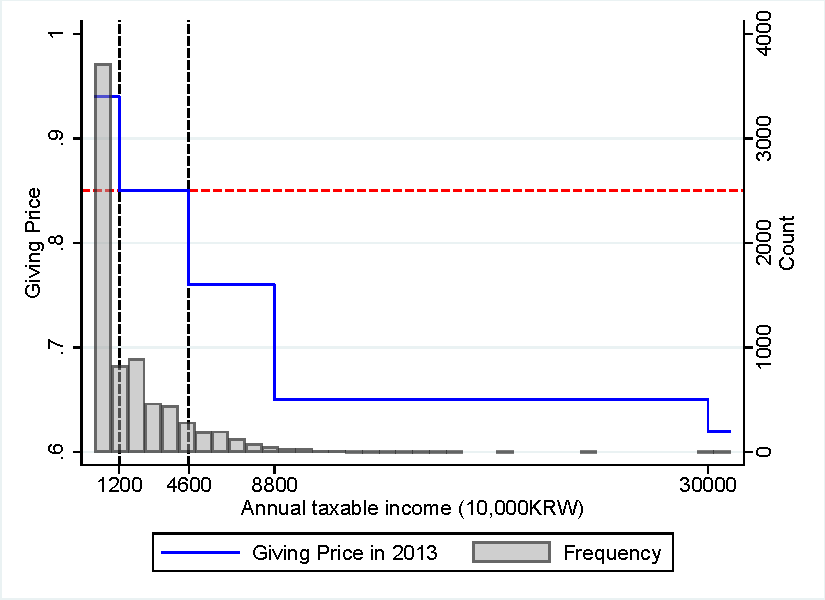
\includegraphics[width=0.9\linewidth]{C:/Users/vge00/Desktop/NaSTaB/_assets/SummaryPriceChange} 
  
  }
  
  \caption{Income Distribution and Giving Price in 2013}\label{fig:showSummaryPriceChange}
  \end{figure}
  
  \hypertarget{estimation}{%
  \section{Estimation}\label{estimation}}
  
  Following Almunia et al. (2020), we estimate giving price elasticity for intensive margin and extensive margin. The elasticity of intensive margin shows how much donors additionally donates reacting to the marginal increase of giving price, while the elasticity of extensive margin shows how much the probability to donate changes reacting to marginal increase of giving price.
  
  We estimate the elasticity of intensive margin using the following specification:
  \[
  \ln g_{it} = \varepsilon_{INT} \ln p_{it} +g_{INT} \ln y_{it} + X_{it}\beta +\mu_i +\iota_t +u_{it}. \label{intensive}
  \]
  \(g_{it}, p_{it}\) and \(y_{it}\) respectively indicates the amount of giving, the giving price, and income of \(i\) in year \(t\). \(\mu_i, \iota_t\) and \(u_{it}\) are individual fixed effect, year fixed effect and error term, respectively.
  The individual fixed effect controls for time-invariant individual characteristics. The year fixed effect controls for events that affect all subjects at the same time. \(X_{it}\) is a vector of covariates which include variables about education and gender. Moreover, we add some interaction terms between year fixed effect and control variables into \(X_{it}\), since they will control for events that affects subject with specific characteristics at the same time following Zeldow and Hatfield (2019).
  
  The elasticity of extensive margin is estimated using the linear probability model such as
  \[
  D_{it} =  \delta \ln p_{it} +\gamma \ln y_{it} + X_{it}\beta+\mu_i  +\iota_t +v_{it}. \label{extensive}
  \]
  \(D_{it}\) is a dummy variable taking 1 if individual \(i\) donates at year \(t\) and 0 otherwise.
  \color{red} Since we use the linear probability model,
  the estimated coefficient \(\delta\) represents \(\hat{\delta} = \frac{\partial D_{it}}{\partial p_{it}} p_{it}\).
  Also, the estimated coefficient \(\gamma\) represents \(\hat{\gamma} = \frac{\partial D_{it}}{\partial y_{it}} y_{it}\).
  Thus, the extensive-margin price and income elasticity are \(\hat{\delta}/D_{it}\) and \(\hat{gamma}/D_{it}\), respectively.
  We evaluate the extensive-margin price and income elasticity at sample mean of \(D_{it}\).
  
  Our identification assumption is the \emph{within} price variation is exogenous because we use the fixed effect model.
  This assumption may be hold because the major \emph{within} price variation comes from the 2014 tax reform.
  After the 2014 tax reform (the tax credit system), the giving price is constant across individuals and
  there is no room for manipulation by donations and income.
  However, before the 2014 tax reform, the giving price has two potential endogeneity problem:
  (A) endogeneity of giving price and (B) simulatenous determination of income and donations.
  By these two reasons, the \emph{within} prive variation is partly endogenous.
  
  Our identification assumption may violate due to two endogenous problems discussed above.
  To tackle these problems, we take two methods.
  First, the giving price is endogenous because
  the tax payer can reduce their giving price by increasing their amount of donation and shifting themselves to the lower tax bracket in the tax deduction system.
  Since this issue does not happen for the first one unit of donation, whose price (``first price'') cannot be changed by adjusting the donation, we use this first price as the giving price in the estimation.
  The first price is formally defined as the giving price \(p^d_i \equiv 1 − \tau (y_i − g_i)\), evaluated at \(g_i = 0\).
  Moreover, this issue does not happen in the tax credit system because the giving price in the tax credit system is exogenously determined by the rate of tax credit allowance.
  Therefore, we construct the giving price in the tax credit system based on the rate of tax credit allowance.
  
  The second issue is simulatenous determination of income and donations.
  Under the tax deduction system,
  the change of income have effects on both donations through the income effect and the giving price through the marginal tax rate.
  Therefore, we employ lagged values of taxable income and construct a variable for the change in the first price of giving as following:
  
  \[
  \ln \left(\frac{p_{it}(y_{it-k} - g_{it-k})}{p_{it-k}(y_{it-k} - g_{it-k})}\right).
  \]
  
  where \(g_{it-k} = 0\).
  The numerator is the first price that individual \(i\) would have faced in year \(t\) if she had declared her year (t − k) taxable income at that year.
  By fixing the income at year \(t - k\),
  the instrument isolates changes in price from income responses to the tax reform.
  Note that this problem does not happen for the tax credit system, where the giving price is the same across all individuals.
  
  \hypertarget{main-results}{%
  \section{Main Results}\label{main-results}}
  
  \hypertarget{price-and-income-elasticity}{%
  \subsection{Price and Income Elasticity}\label{price-and-income-elasticity}}
  
  \begin{itemize}
  \tightlist
  \item
    To show our baseline results graphically, Figure \ref{fig:showElasticityResid} shows average residuals grouped by year and benefit of the 2014 tax reform.
  
    \begin{itemize}
    \tightlist
    \item
      Residuals are obtained from the regression of logged donations on logged annual taxable income, individual and time fixed year.
    \end{itemize}
  \end{itemize}
  
  \hypertarget{price-and-income-elasticity-residuals-plot}{%
  \subsection{Price and Income Elasticity: Residuals Plot}\label{price-and-income-elasticity-residuals-plot}}
  
  Those who incurring loss owing to the 2014 tax reform drastically decreases thier amount of donations.
  
  \begin{figure}
  
  {\centering 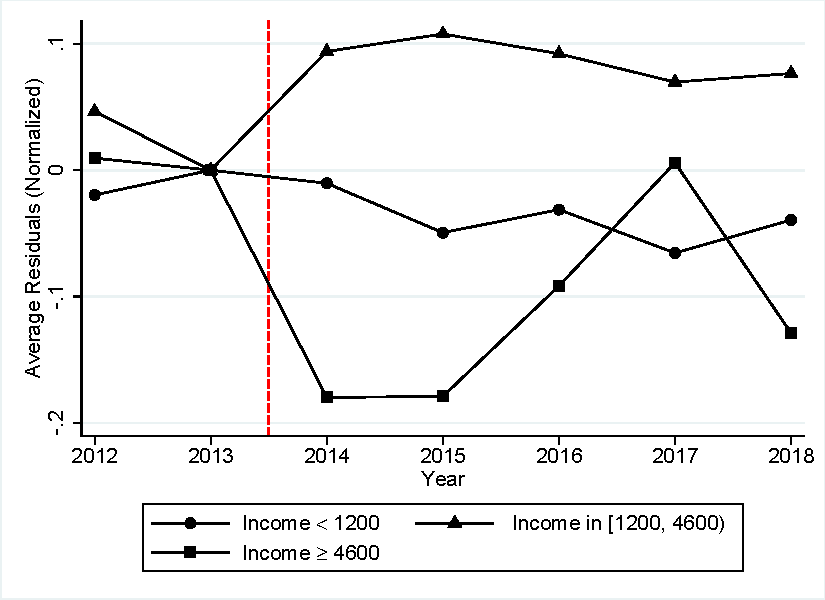
\includegraphics[width=0.8\linewidth]{C:/Users/vge00/Desktop/NaSTaB/_assets/ElasticityResid} 
  
  }
  
  \caption{Average Residuals Grouped by Year and Tax-Reform Benefit Group}\label{fig:showElasticityResid}
  \end{figure}
  
  \hypertarget{price-and-income-elasticity-estimation-results}{%
  \subsection{Price and Income Elasticity: Estimation Results}\label{price-and-income-elasticity-estimation-results}}
  
  We found the \textbf{price effect} of giving (1\% price increase leads to about 1.1\% giving decrease),
  and the \textbf{income effect} of giving(1\% income increase leads to about 5\% giving increase).
  
  \begin{table}
  
  \caption{\label{tab:kableEstimateElasticityPart1}Main Results}
  \centering
  \fontsize{7}{9}\selectfont
  \begin{tabular}[t]{lccccc}
  \toprule
   & (1) & (2) & (3) & (4) & (5)\\
  \midrule
  ln(giving price) & -1.072*** & -1.264*** & -1.291*** & -1.114*** & -1.241***\\
   & (0.202) & (0.213) & (0.230) & (0.229) & (0.227)\\
  ln(auunaul taxable income) & 5.392*** & 5.080*** & 5.047*** & 5.116*** & 4.946***\\
   & (0.970) & (0.964) & (0.964) & (0.966) & (0.949)\\
  Age & N & Y & Y & Y & Y\\
  Year X Education & N & N & Y & Y & Y\\
  Year X Gender & N & N & N & Y & Y\\
  Year X Resident Area & N & N & N & N & Y\\
  N & 53269 & 53269 & 53267 & 53267 & 53267\\
  \bottomrule
  \end{tabular}
  \end{table}
  
  \hypertarget{intensive-and-extensive-margin}{%
  \subsection{Intensive and Extensive Margin}\label{intensive-and-extensive-margin}}
  
  \begin{itemize}
  \tightlist
  \item
    To obtain intensive- and extensive-margin elasticity, we repeat the same excercise.
  \item
    Figure \ref{fig:showIntElasticityResid} shows average residuals grouped by year and benefit of the 2014 tax reform
  
    \begin{itemize}
    \tightlist
    \item
      We used those who donated and estimated residuals obtained from the regression logged donations on logged annual taxable income, individual and time fixed year.
    \end{itemize}
  \item
    Figure \ref{fig:showExtElasticityResid} shows average residuals grouped by year and benefir of the 2014 tax reform.
  
    \begin{itemize}
    \tightlist
    \item
      We estimated residuals obtained from the regression the donation dummy on logged annual taxable income, individual and time fixed year.
    \end{itemize}
  \end{itemize}
  
  \hypertarget{intensive-margin-residuals-plot}{%
  \subsection{Intensive Margin: Residuals Plot}\label{intensive-margin-residuals-plot}}
  
  Donors who receive benefit owing to the 2014 tax reform decrease their donations in 2014 and 2015.
  
  \begin{figure}
  
  {\centering 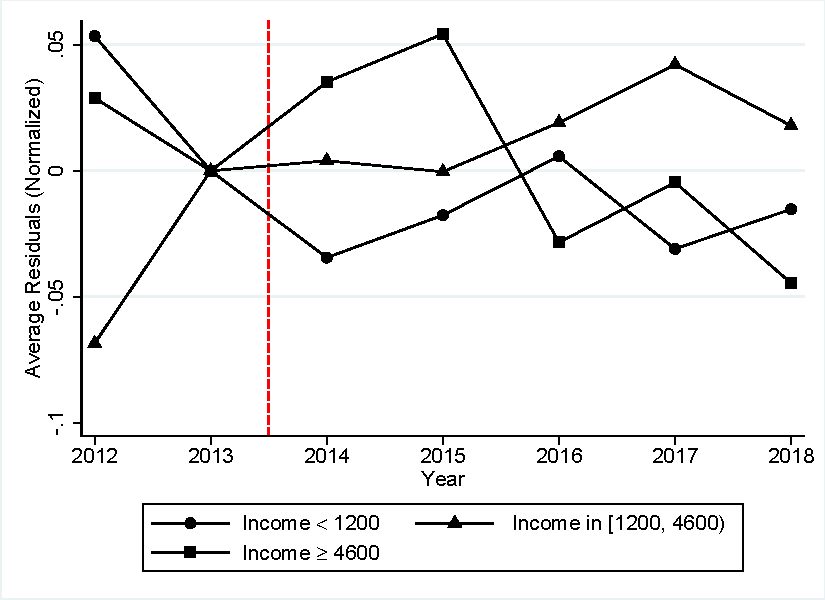
\includegraphics[width=0.8\linewidth]{C:/Users/vge00/Desktop/NaSTaB/_assets/IntElasticityResid} 
  
  }
  
  \caption{Average Residuals Grouped by Year and Tax-Reform Benefit Group (Intensive Margin)}\label{fig:showIntElasticityResid}
  \end{figure}
  
  \hypertarget{extensive-margin-residuals-plot}{%
  \subsection{Extensive Margin: Residuals Plot}\label{extensive-margin-residuals-plot}}
  
  Those who incurring loss owing to the 2014 tax reform drastically were less likely to donate.
  
  \begin{figure}
  
  {\centering 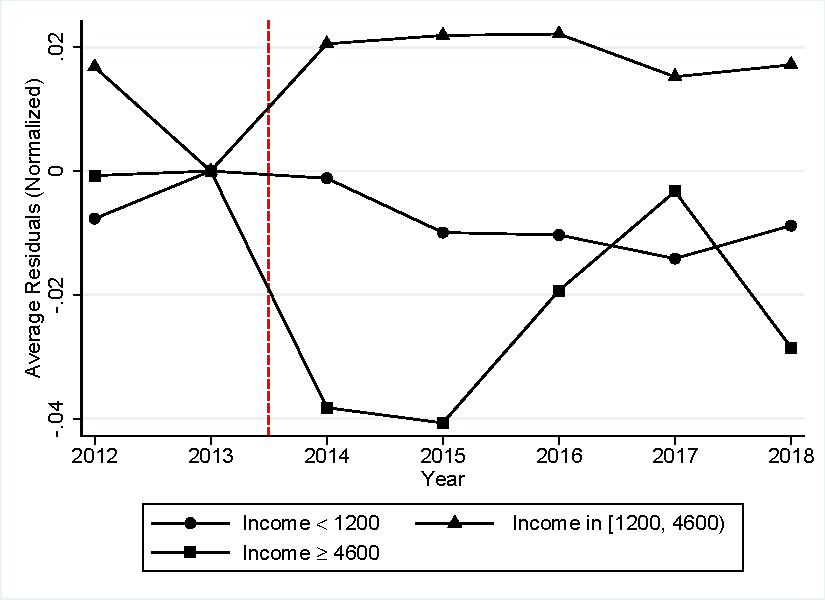
\includegraphics[width=0.8\linewidth]{C:/Users/vge00/Desktop/NaSTaB/_assets/ExtElasticityResid} 
  
  }
  
  \caption{Average Residuals Grouped by Year and Tax-Reform Benefit Group (Extensive Margin)}\label{fig:showExtElasticityResid}
  \end{figure}
  
  \hypertarget{intensive-and-extensive-margin-estimation-results}{%
  \subsection{Intensive and Extensive Margin: Estimation Results}\label{intensive-and-extensive-margin-estimation-results}}
  
  The intensive-margin price elasticity is -0.5 \textasciitilde{} -1\%.
  
  \begin{table}
  
  \caption{\label{tab:kableEstimateElasticityPart2Slide1}Main Results: Intensive-Margin Elasticity}
  \centering
  \fontsize{7}{9}\selectfont
  \begin{tabular}[t]{lccccc}
  \toprule
   & (1) & (2) & (3) & (4) & (5)\\
  \midrule
  ln(giving price) & -0.593*** & -0.838*** & -1.016*** & -0.893*** & -0.904***\\
   & (0.203) & (0.212) & (0.232) & (0.243) & (0.248)\\
  ln(auunaul taxable income) & 2.015*** & 1.562** & 1.445** & 1.528** & 1.571**\\
   & (0.675) & (0.655) & (0.647) & (0.651) & (0.653)\\
  Age & N & Y & Y & Y & Y\\
  Year X Education & N & N & Y & Y & Y\\
  Year X Gender & N & N & N & Y & Y\\
  Year X Resident Area & N & N & N & N & Y\\
  N & 11637 & 11637 & 11637 & 11637 & 11637\\
  \bottomrule
  \end{tabular}
  \end{table}
  
  \hypertarget{intensive-and-extensive-margin-estimation-results-1}{%
  \subsection{Intensive and Extensive Margin: Estimation Results}\label{intensive-and-extensive-margin-estimation-results-1}}
  
  The extensive-margin price elasticity is -1.2 \textasciitilde{} -1.4\%.
  
  \begin{table}
  
  \caption{\label{tab:kableEstimateElasticityPart2Slide2}Main Results: Extensive-Margin Elasticity}
  \centering
  \fontsize{7}{9}\selectfont
  \begin{tabular}[t]{lccccc}
  \toprule
   & (1) & (2) & (3) & (4) & (5)\\
  \midrule
  Implied price elasiticity & -1.264*** & -1.418*** & -1.343*** & -1.167*** & -1.312***\\
   & (0.226) & (0.237) & (0.256) & (0.256) & (0.253)\\
  Implied income elasticity & 5.778*** & 5.527*** & 5.531*** & 5.600*** & 5.420***\\
   & (1.099) & (1.097) & (1.099) & (1.100) & (1.080)\\
  Age & N & Y & Y & Y & Y\\
  Year X Education & N & N & Y & Y & Y\\
  Year X Gender & N & N & N & Y & Y\\
  Year X Resident Area & N & N & N & N & Y\\
  N & 53269 & 53269 & 53267 & 53267 & 53267\\
  \bottomrule
  \end{tabular}
  \end{table}
  
  \hypertarget{robustness-check-1}{%
  \subsection{Robustness Check 1}\label{robustness-check-1}}
  
  First potential concern: last price elasticity
  
  \begin{itemize}
  \tightlist
  \item
    Our baseline results show the \textbf{first} price elasticity to avoid the endogeneity of giving price.
  \item
    We estimated the \textbf{last} price elasticity, using the Panel IV method.
  
    \begin{itemize}
    \tightlist
    \item
      The instrument is the first giving price.
    \item
      Note that the last giving price is equal to the first giving price under the tax credit system.
    \end{itemize}
  \end{itemize}
  
  \hypertarget{robustness-check-1-result}{%
  \subsection{Robustness Check 1: Result}\label{robustness-check-1-result}}
  
  Overall last price elasticity increases twofold.
  
  \begin{table}
  
  \caption{\label{tab:kableLastElasticity1}Last Price Elasticity: Panel IV}
  \centering
  \fontsize{7}{9}\selectfont
  \begin{tabular}[t]{lccccc}
  \toprule
   & (1) & (2) & (3) & (4) & (5)\\
  \midrule
  ln(last giving price) & -2.421*** & -2.536*** & -2.750*** & -2.529*** & -2.650***\\
   & (0.204) & (0.216) & (0.233) & (0.231) & (0.229)\\
  ln(auunaul taxable income) & 5.258*** & 5.071*** & 4.981*** & 5.058*** & 4.910***\\
   & (0.961) & (0.961) & (0.959) & (0.961) & (0.948)\\
  Age & N & Y & Y & Y & Y\\
  Year X Education & N & N & Y & Y & Y\\
  Year X Gender & N & N & N & Y & Y\\
  Year X Resident Area & N & N & N & N & Y\\
  N & 52304 & 52304 & 52302 & 52302 & 52302\\
  \bottomrule
  \end{tabular}
  \end{table}
  
  \hypertarget{robustness-check-1-intensive-margin}{%
  \subsection{Robustness Check 1: Intensive Margin}\label{robustness-check-1-intensive-margin}}
  
  The intensive-margin last price elasticity lies within the range of the first price elasticity.
  
  \begin{table}
  
  \caption{\label{tab:kableLastElasticity2Slide1}Intensive-Margin Last Price Elasticity: Panel IV}
  \centering
  \fontsize{7}{9}\selectfont
  \begin{tabular}[t]{lccccc}
  \toprule
   & (1) & (2) & (3) & (4) & (5)\\
  \midrule
  ln(last giving price) & -0.898*** & -0.961*** & -1.197*** & -0.998*** & -1.074***\\
   & (0.271) & (0.271) & (0.307) & (0.325) & (0.332)\\
  ln(auunaul taxable income) & 2.023*** & 1.638** & 1.460** & 1.530** & 1.572**\\
   & (0.694) & (0.678) & (0.667) & (0.670) & (0.667)\\
  Age & N & Y & Y & Y & Y\\
  Year X Education & N & N & Y & Y & Y\\
  Year X Gender & N & N & N & Y & Y\\
  Year X Resident Area & N & N & N & N & Y\\
  N & 10672 & 10672 & 10672 & 10672 & 10672\\
  \bottomrule
  \end{tabular}
  \end{table}
  
  \hypertarget{robustness-check-1-extensive-margin}{%
  \subsection{Robustness Check 1: Extensive Margin}\label{robustness-check-1-extensive-margin}}
  
  The extensive-margin last price elasticity at sample mean is roughly -3\%.
  
  \begin{table}
  
  \caption{\label{tab:kableLastElasticity2Slide2}Extensive-Margin Last Price Elasticity: Panel IV}
  \centering
  \fontsize{7}{9}\selectfont
  \begin{tabular}[t]{lccccc}
  \toprule
   & (1) & (2) & (3) & (4) & (5)\\
  \midrule
  Implied last price elasiticity & -3.063*** & -3.100*** & -3.167*** & -2.917*** & -3.046***\\
   & (0.227) & (0.240) & (0.259) & (0.258) & (0.254)\\
  Implied income elasticity & 5.532*** & 5.472*** & 5.426*** & 5.513*** & 5.361***\\
   & (1.088) & (1.096) & (1.096) & (1.098) & (1.082)\\
  Age & N & Y & Y & Y & Y\\
  Year X Education & N & N & Y & Y & Y\\
  Year X Gender & N & N & N & Y & Y\\
  Year X Resident Area & N & N & N & N & Y\\
  N & 52304 & 52304 & 52302 & 52302 & 52302\\
  \bottomrule
  \end{tabular}
  \end{table}
  
  \hypertarget{robust-check-2}{%
  \subsection{Robust Check 2}\label{robust-check-2}}
  
  Second potential concern: Price change due to the change of income
  
  \begin{itemize}
  \tightlist
  \item
    Since the giving price under the tax deduction depends on the change of income, the \emph{within} variation of giving price may be endogenous.
  \item
    To resolve this concern, we used the data (i) from 2013 to 2018 or (ii) from 2013 to 2014, and estimated the fixed effect model.
  
    \begin{itemize}
    \tightlist
    \item
      By this restriction, the \emph{within} price variation of giving price is completely exgonenous.
    \end{itemize}
  \end{itemize}
  
  \hypertarget{robustness-check-2-result}{%
  \subsection{Robustness Check 2: Result}\label{robustness-check-2-result}}
  
  Overall price elasticity is -1 \textasciitilde{} -1.7\%.
  
  \begin{table}
  
  \caption{\label{tab:kableShortElasticity1}Elasticity with Short-Period Data}
  \centering
  \fontsize{8}{10}\selectfont
  \begin{tabular}[t]{lcccc}
  \toprule
  \multicolumn{1}{c}{ } & \multicolumn{2}{c}{After 2012} & \multicolumn{2}{c}{2013 and 2014} \\
  \cmidrule(l{3pt}r{3pt}){2-3} \cmidrule(l{3pt}r{3pt}){4-5}
   & (1) & (2) & (3) & (4)\\
  \midrule
  ln(giving price) & -1.014*** & -1.286*** & -1.398*** & -1.686***\\
   & (0.255) & (0.290) & (0.289) & (0.338)\\
  ln(auunaul taxable income) & 5.108*** & 4.743*** & 4.013** & 3.035\\
   & (1.009) & (0.990) & (1.948) & (1.992)\\
  Other Controls & N & Y & N & Y\\
  N & 45994 & 45992 & 14893 & 14893\\
  \bottomrule
  \end{tabular}
  \end{table}
  
  \hypertarget{robustness-check-2-intensive-marign}{%
  \subsection{Robustness Check 2: Intensive Marign}\label{robustness-check-2-intensive-marign}}
  
  The intensive-margin price elasticity is -0.6 \textasciitilde{} -1\%.
  In column (3), the price elasticity is statistically insignificant.
  
  \begin{table}
  
  \caption{\label{tab:kableShortElasticity2Slide1}Intensive-Margin Elasticity with Short-Period Data}
  \centering
  \fontsize{8}{10}\selectfont
  \begin{tabular}[t]{lcccc}
  \toprule
  \multicolumn{1}{c}{ } & \multicolumn{2}{c}{After 2012} & \multicolumn{2}{c}{2013 and 2014} \\
  \cmidrule(l{3pt}r{3pt}){2-3} \cmidrule(l{3pt}r{3pt}){4-5}
   & (1) & (2) & (3) & (4)\\
  \midrule
  ln(giving price) & -0.647*** & -1.129*** & -0.394 & -0.712**\\
   & (0.236) & (0.291) & (0.310) & (0.363)\\
  ln(auunaul taxable income) & 1.943*** & 1.714*** & 1.440 & 1.047\\
   & (0.662) & (0.649) & (2.975) & (3.072)\\
  Other Controls & N & Y & N & Y\\
  N & 10158 & 10158 & 2922 & 2922\\
  \bottomrule
  \end{tabular}
  \end{table}
  
  \hypertarget{robustness-check-2-extensive-marign}{%
  \subsection{Robustness Check 2: Extensive Marign}\label{robustness-check-2-extensive-marign}}
  
  The extensive-margin price elasticity at sample mean is -1 \textasciitilde{} -2\%.
  
  \begin{table}
  
  \caption{\label{tab:kableShortElasticity2Slide2}Extensive-Margin Elasticity with Short-Period Data}
  \centering
  \fontsize{8}{10}\selectfont
  \begin{tabular}[t]{lcccc}
  \toprule
  \multicolumn{1}{c}{ } & \multicolumn{2}{c}{After 2012} & \multicolumn{2}{c}{2013 and 2014} \\
  \cmidrule(l{3pt}r{3pt}){2-3} \cmidrule(l{3pt}r{3pt}){4-5}
   & (1) & (2) & (3) & (4)\\
  \midrule
  Implied price elasiticity & -1.136*** & -1.300*** & -1.845*** & -2.131***\\
   & (0.279) & (0.314) & (0.364) & (0.422)\\
  Implied income elasticity & 5.287*** & 4.954*** & 4.457* & 3.196\\
   & (1.114) & (1.094) & (2.381) & (2.488)\\
  Other Controls & N & Y & N & Y\\
  N & 45994 & 45992 & 14893 & 14893\\
  \bottomrule
  \end{tabular}
  \end{table}
  
  \hypertarget{robustness-check-3}{%
  \subsection{Robustness Check 3}\label{robustness-check-3}}
  
  Second potential concerns: the change of price due to the change of income
  
  \begin{itemize}
  \tightlist
  \item
    To exclude this potential concerns, previous identification strategy uses the 2014 tax reform.
  \item
    We can also rule out this problem, using the change in the first giving price.
  
    \begin{itemize}
    \tightlist
    \item
      The change in the first giving price is \(\ln(p_{it}(y_{it-k} - g_{it-k})/p_{it-k}(y_{it-k} - g_{it-k}))\) where \(g_{it-k} = 0\).
    \item
      Since we fix the income \(y_{it-k}\), this variation comes from the tax reform.
    \end{itemize}
  \end{itemize}
  
  \hypertarget{robustness-check-3-contd}{%
  \subsection{Robustness Check 3 (Cont'd)}\label{robustness-check-3-contd}}
  
  Our estimation equation is
  \[\Delta^k \ln g_{it} = \delta \Delta^k \ln p_{it} + \gamma \Delta^k \ln y_{it} + \Delta^k X_{it} \beta + \mu_i + \iota_t + v_{it},\]
  where \(\Delta^k Y_{it} = Y_{it} - Y_{it-k}\).
  
  \begin{itemize}
  \tightlist
  \item
    Note that we cannot estimation the extensive-margin elasticity since it is hard to interapt this estimation equation when we use \(\Delta^k D_{it}\) as an outcome.
  \item
    We estimate this model for \(k = 1, 2, 3\).
  \end{itemize}
  
  \hypertarget{robustness-check-3-overall-elasticity}{%
  \subsection{Robustness Check 3: Overall Elasticity}\label{robustness-check-3-overall-elasticity}}
  
  Overall price elasticity is rougnly -2\%.
  
  \begin{table}
  
  \caption{\label{tab:kablekDiffElasticitySlide1}Overall Elasticity: $k$-difference model}
  \centering
  \fontsize{8}{10}\selectfont
  \begin{tabular}[t]{lccc}
  \toprule
  \multicolumn{1}{c}{lag $k$} & \multicolumn{1}{c}{$k = 1$} & \multicolumn{1}{c}{$k = 2$} & \multicolumn{1}{c}{$k = 3$} \\
  \cmidrule(l{3pt}r{3pt}){1-1} \cmidrule(l{3pt}r{3pt}){2-2} \cmidrule(l{3pt}r{3pt}){3-3} \cmidrule(l{3pt}r{3pt}){4-4}
   & (1) & (2) & (3)\\
  \midrule
  Lagged difference of first price (log) & -1.894*** & -2.170*** & -1.752***\\
   & (0.389) & (0.355) & (0.346)\\
  Lagged difference of annual income (log) & 2.737*** & 4.685*** & 5.307***\\
   & (1.042) & (1.141) & (1.174)\\
  N & 49014 & 46610 & 44205\\
  \bottomrule
  \end{tabular}
  \end{table}
  
  \hypertarget{robustness-check-3-intensive-margin-elasticity}{%
  \subsection{Robustness Check 3: Intensive-Margin Elasticity}\label{robustness-check-3-intensive-margin-elasticity}}
  
  The intensive-margin price elasticity is rougnly -2\%.
  
  \begin{table}
  
  \caption{\label{tab:kablekDiffElasticitySlide2}Intensive-Margin Elasticity: $k$-difference model}
  \centering
  \fontsize{8}{10}\selectfont
  \begin{tabular}[t]{lccc}
  \toprule
  \multicolumn{1}{c}{lag $k$} & \multicolumn{1}{c}{$k = 1$} & \multicolumn{1}{c}{$k = 2$} & \multicolumn{1}{c}{$k = 3$} \\
  \cmidrule(l{3pt}r{3pt}){1-1} \cmidrule(l{3pt}r{3pt}){2-2} \cmidrule(l{3pt}r{3pt}){3-3} \cmidrule(l{3pt}r{3pt}){4-4}
   & (1) & (2) & (3)\\
  \midrule
  Lagged difference of first price (log) & -1.854** & -2.282*** & -2.163***\\
   & (0.763) & (0.621) & (0.550)\\
  Lagged difference of annual income (log) & 2.229 & 4.675*** & 5.582**\\
   & (1.715) & (1.791) & (2.178)\\
  N & 10939 & 10505 & 10043\\
  \bottomrule
  \end{tabular}
  \end{table}
  
  \hypertarget{governement-efficient-and-price-elasticity}{%
  \section{Governement Efficient and Price Elasticity}\label{governement-efficient-and-price-elasticity}}
  
  \hypertarget{construct-efficiency-index}{%
  \subsection{Construct Efficiency Index}\label{construct-efficiency-index}}
  
  From the 2015 survey, NaSTaB asks the current and ideal balance between tax burden and welfare level.
  See the following table.
  
  \begin{table}[H]
  \centering\begingroup\fontsize{8}{10}\selectfont
  
  \begin{tabular}{l|cccl|cccl|cccl|ccc}
  \toprule
  Welfare/Tax burden & Low & Middle & High\\
  \midrule
  High & 2 & 1 & 0\\
  Middle & 1 & 0 & -1\\
  Low & 0 & -1 & 2\\
  \bottomrule
  \end{tabular}
  \endgroup{}
  \end{table}
  
  \hypertarget{construct-efficient-index-contd}{%
  \subsection{Construct Efficient Index (Cont'd)}\label{construct-efficient-index-contd}}
  
  \begin{itemize}
  \tightlist
  \item
    The pair of answers reflect the individual's perception about the efficiency of government because the government with low tax burden and high welfare level is clearly more efficient than one with high tax and low welfare.
  \item
    Based on the pair about current perception, we construct an index called efficiency index by the following steps.
  
    \begin{enumerate}
    \def\labelenumi{\arabic{enumi}.}
    \tightlist
    \item
      We assign the number from -2 to 2 for each pair of answers depending on the contents of answers, where -2 is the most inefficient and 2 is the most efficient.
    \item
      To construct the individual's persistent perception toward the government, we regress the assigned number on year fixed effect, the interaction between region and year fixed effect, and individual fixed effect.
    \item
      use the obtained fixed effect as the efficiency index
    \end{enumerate}
  \end{itemize}
  
  \hypertarget{histrogram-of-efficient-index}{%
  \subsection{Histrogram of Efficient Index}\label{histrogram-of-efficient-index}}
  
  \begin{figure}
  
  {\centering 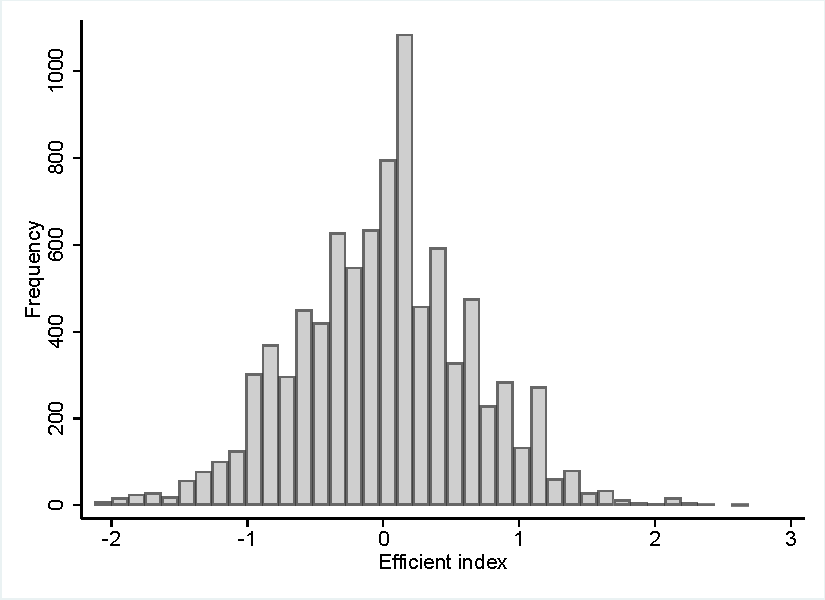
\includegraphics[width=0.9\linewidth]{C:/Users/vge00/Desktop/NaSTaB/_assets/HistogramEfficientid} 
  
  }
  
  \caption{Histogram of Efficient Index}\label{fig:unnamed-chunk-1}
  \end{figure}
  
  \hypertarget{two-potential-concerns}{%
  \subsection{Two Potential Concerns}\label{two-potential-concerns}}
  
  \begin{enumerate}
  \def\labelenumi{\arabic{enumi}.}
  \tightlist
  \item
    There is a room for subjects to interpret the questions of tax/welfare balance as questions about the expenditure policy of the government.
  
    \begin{itemize}
    \tightlist
    \item
      To address this issue, we use the question for ideal balance between tax burden and welfare level to rule out the subjects who consider that the higher welfare level than the tax burden is unfavorable.
    \end{itemize}
  \item
    Efficiency indexの構成方法にかかわる問題をここに書こうかと思います。上記では固定効果をとっている理由をPersistentな政府へのperceptionを見たいからとしていますが、別にそれぞれの時点でのperceptionをとっても構わないだろうとツッコミが来ると思うので、なぜ固定効果をとっているのかなどを書いてもらえればと思います。
  \end{enumerate}
  
  \hypertarget{heterogenous-price-elasticity-by-governement-efficiency}{%
  \subsection{Heterogenous Price Elasticity by Governement Efficiency}\label{heterogenous-price-elasticity-by-governement-efficiency}}
  
  To see the heterogenous price elasticity by efficient index,
  we utilize the interaction between the efficiency index and the giving price.
  
  Bothe ways of the analyses use the sepcifications based on the Equation (XX) and (XX) for intensive and extensive margins,
  respectively.
  
  We control individual and time fixed effect,
  and other covariates.
  
  \hypertarget{heterogenous-price-elasticity-estimations-results}{%
  \subsection{Heterogenous Price Elasticity: Estimations Results}\label{heterogenous-price-elasticity-estimations-results}}
  
  \begin{table}
  
  \caption{\label{tab:kableHeteroElasticitySlide1}Heterogenous Elasticity by Perceived Government Efficiency (1)}
  \centering
  \fontsize{8}{10}\selectfont
  \begin{tabular}[t]{lccc}
  \toprule
  \multicolumn{1}{c}{ } & \multicolumn{1}{c}{Overall} & \multicolumn{1}{c}{Extensive} & \multicolumn{1}{c}{Intensive} \\
  \cmidrule(l{3pt}r{3pt}){2-2} \cmidrule(l{3pt}r{3pt}){3-3} \cmidrule(l{3pt}r{3pt}){4-4}
   & (1) & (2) & (3)\\
  \midrule
  ln(giving price) & -1.356*** & -0.284*** & -0.952***\\
   & (0.336) & (0.076) & (0.334)\\
  ln(giving price) X 2Q Efficient Group & -0.032 & -0.059 & 0.292\\
   & (0.423) & (0.098) & (0.489)\\
  ln(giving price) X 3Q Efficient Group & 0.353 & 0.095 & -0.285\\
   & (0.417) & (0.097) & (0.545)\\
  N & 50455 & 50455 & 11327\\
  \bottomrule
  \end{tabular}
  \end{table}
  
  \hypertarget{heterogenous-price-elasticity-implied-elasticity}{%
  \subsection{Heterogenous Price Elasticity: Implied Elasticity}\label{heterogenous-price-elasticity-implied-elasticity}}
  
  \begin{table}
  
  \caption{\label{tab:kableHeteroElasticitySlide2}Heterogenous Elasticity by Perceived Government Efficiency (2)}
  \centering
  \fontsize{8}{10}\selectfont
  \begin{tabular}[t]{lccc}
  \toprule
  \multicolumn{1}{c}{ } & \multicolumn{1}{c}{Overall} & \multicolumn{1}{c}{Extensive} & \multicolumn{1}{c}{Intensive} \\
  \cmidrule(l{3pt}r{3pt}){2-2} \cmidrule(l{3pt}r{3pt}){3-3} \cmidrule(l{3pt}r{3pt}){4-4}
   & (1) & (2) & (3)\\
  \midrule
  Implied price elasiticity (1Q efficient group) & -1.356*** & -1.396*** & -0.952***\\
   & (0.336) & (0.374) & (0.334)\\
  Implied price elasiticity (2Q efficient group) & -1.388*** & -1.686*** & -0.661*\\
   & (0.330) & (0.378) & (0.394)\\
  Implied price elasiticity (3Q efficient group) & -1.002*** & -0.930** & -1.237***\\
   & (0.327) & (0.374) & (0.468)\\
  N & 50455 & 50455 & 11327\\
  \bottomrule
  \end{tabular}
  \end{table}
  
  \hypertarget{robustness-check-1-1}{%
  \subsection{Robustness Check 1}\label{robustness-check-1-1}}
  
  First Potential Concern: interpretaion of the questions of tax/welfare balance as questions about the expenditure policy of the government
  
  \begin{itemize}
  \tightlist
  \item
    First, we construct three quantile groups, using the original efficient index.
  \item
    Second, we rule out the subjects whose efficiency index for the ideal balance question is less than 0 from each group.
  \end{itemize}
  
  \hypertarget{robustness-check-1-density-of-efficient-index}{%
  \subsection{Robustness Check 1: Density of Efficient Index}\label{robustness-check-1-density-of-efficient-index}}
  
  \begin{figure}
  
  {\centering 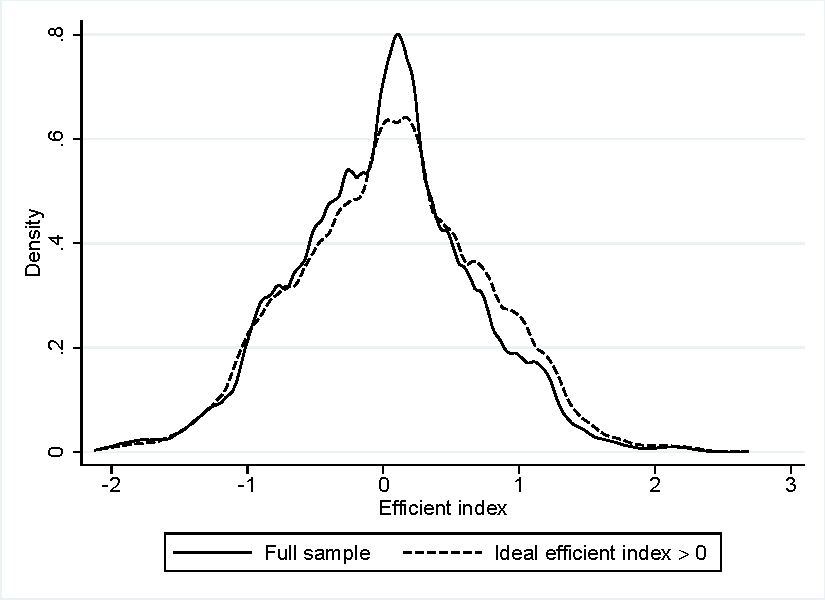
\includegraphics[width=0.9\linewidth]{C:/Users/vge00/Desktop/NaSTaB/_assets/DensityEfficientid} 
  
  }
  
  \caption{Density of Efficient Index Using those whose ideal efficient index > 0}\label{fig:unnamed-chunk-2}
  \end{figure}
  
  \hypertarget{robustness-check-1-estimation-results}{%
  \subsection{Robustness Check 1: Estimation Results}\label{robustness-check-1-estimation-results}}
  
  \begin{table}
  
  \caption{\label{tab:kableSubsetHeteroElasticitySlide1}Heterogenous Elasticity Using Those whose Ideal Efficient Index > 0 (1)}
  \centering
  \fontsize{8}{10}\selectfont
  \begin{tabular}[t]{lccc}
  \toprule
   & (1) & (2) & (3)\\
  \midrule
  ln(giving price) & -1.831*** & -0.316*** & -1.303**\\
   & (0.538) & (0.115) & (0.571)\\
  ln(giving price) X 2Q Efficient Group & 0.339 & 0.045 & 0.308\\
   & (0.657) & (0.146) & (0.807)\\
  ln(giving price) X 3Q Efficient Group & 1.295** & 0.237* & 0.236\\
   & (0.586) & (0.135) & (0.834)\\
  N & 23366 & 23366 & 5004\\
  \bottomrule
  \end{tabular}
  \end{table}
  
  \hypertarget{robustness-check-1-implied-price-elasticity}{%
  \subsection{Robustness Check 1: Implied Price Elasticity}\label{robustness-check-1-implied-price-elasticity}}
  
  \begin{table}
  
  \caption{\label{tab:kableSubsetHeteroElasticitySlide2}Heterogenous Elasticity Using Those whose Ideal Efficient Index > 0 (1)}
  \centering
  \fontsize{8}{10}\selectfont
  \begin{tabular}[t]{lccc}
  \toprule
   & (1) & (2) & (3)\\
  \midrule
  Implied price elasiticity (1Q efficient group) & -1.831*** & -1.555*** & -1.303**\\
   & (0.538) & (0.565) & (0.571)\\
  Implied price elasiticity (2Q efficient group) & -1.492*** & -1.335** & -0.995\\
   & (0.505) & (0.561) & (0.622)\\
  Implied price elasiticity (3Q efficient group) & -0.536 & -0.392 & -1.067\\
   & (0.416) & (0.500) & (0.680)\\
  N & 23366 & 23366 & 5004\\
  \bottomrule
  \end{tabular}
  \end{table}
  
  \hypertarget{robustness-check-2}{%
  \subsection{Robustness Check 2}\label{robustness-check-2}}
  
  Second potential concern: Last price elasticity
  
  \begin{itemize}
  \tightlist
  \item
    We repeat same excercise as the panel IV including two interaction terms as endogenous variables.
  \item
    Exgonenous variables are the interaction between giving price and dummies of efficient index group.
  \end{itemize}
  
  \hypertarget{robustness-check-2-estimation-results-1}{%
  \subsection{Robustness Check 2: Estimation Results (1)}\label{robustness-check-2-estimation-results-1}}
  
  \begin{table}
  
  \caption{\label{tab:kableHeteroLastElasticitySlide1}Heterogenous Last Price Elasticity: Panel IV (1)}
  \centering
  \fontsize{8}{10}\selectfont
  \begin{tabular}[t]{lccc}
  \toprule
  \multicolumn{1}{c}{ } & \multicolumn{3}{c}{Full Sample} \\
  \cmidrule(l{3pt}r{3pt}){2-4}
  \multicolumn{1}{c}{ } & \multicolumn{1}{c}{Overall} & \multicolumn{1}{c}{Extensive} & \multicolumn{1}{c}{Intensive} \\
  \cmidrule(l{3pt}r{3pt}){2-2} \cmidrule(l{3pt}r{3pt}){3-3} \cmidrule(l{3pt}r{3pt}){4-4}
   & (1) & (2) & (3)\\
  \midrule
  ln(last giving price) & -2.604*** & -0.586*** & -1.166***\\
   & (0.342) & (0.077) & (0.438)\\
  ln(last giving price) X 2Q Efficient Group & -0.272 & -0.104 & 0.043\\
   & (0.417) & (0.095) & (0.591)\\
  ln(last giving price) X 3Q Efficient Group & -0.010 & -0.038 & 0.111\\
   & (0.420) & (0.096) & (0.709)\\
  N & 49575 & 49575 & 10447\\
  \bottomrule
  \end{tabular}
  \end{table}
  
  \hypertarget{robustness-check-2-implied-price-elasticity-1}{%
  \subsection{Robustness Check 2: Implied Price Elasticity (1)}\label{robustness-check-2-implied-price-elasticity-1}}
  
  \begin{table}
  
  \caption{\label{tab:kableHeteroLastElasticitySlide2}Heterogenous Last Price Elasticity: Panel IV (2)}
  \centering
  \fontsize{8}{10}\selectfont
  \begin{tabular}[t]{lccc}
  \toprule
  \multicolumn{1}{c}{ } & \multicolumn{3}{c}{Full Sample} \\
  \cmidrule(l{3pt}r{3pt}){2-4}
  \multicolumn{1}{c}{ } & \multicolumn{1}{c}{Overall} & \multicolumn{1}{c}{Extensive} & \multicolumn{1}{c}{Intensive} \\
  \cmidrule(l{3pt}r{3pt}){2-2} \cmidrule(l{3pt}r{3pt}){3-3} \cmidrule(l{3pt}r{3pt}){4-4}
   & (1) & (2) & (3)\\
  \midrule
  Implied last price elasiticity (1Q efficient group) & -2.604*** & -2.883*** & -1.166***\\
   & (0.342) & (0.377) & (0.438)\\
  Implied last price elasiticity (2Q efficient group) & -2.876*** & -3.395*** & -1.122**\\
   & (0.318) & (0.362) & (0.488)\\
  Implied last price elasiticity (3Q efficient group) & -2.614*** & -3.071*** & -1.055*\\
   & (0.328) & (0.371) & (0.639)\\
  N & 49575 & 49575 & 10447\\
  \bottomrule
  \end{tabular}
  \end{table}
  
  \hypertarget{robustness-check-2-estimation-results-2}{%
  \subsection{Robustness Check 2: Estimation Results (2)}\label{robustness-check-2-estimation-results-2}}
  
  \begin{table}
  
  \caption{\label{tab:kableHeteroLastElasticitySlide3}Heterogenous Last Price Elasticity: Panel IV (3)}
  \centering
  \fontsize{8}{10}\selectfont
  \begin{tabular}[t]{lccc}
  \toprule
  \multicolumn{1}{c}{ } & \multicolumn{3}{c}{Ideal Efficient Index > 0} \\
  \cmidrule(l{3pt}r{3pt}){2-4}
  \multicolumn{1}{c}{ } & \multicolumn{1}{c}{Overall} & \multicolumn{1}{c}{Extensive} & \multicolumn{1}{c}{Intensive} \\
  \cmidrule(l{3pt}r{3pt}){2-2} \cmidrule(l{3pt}r{3pt}){3-3} \cmidrule(l{3pt}r{3pt}){4-4}
   & (4) & (5) & (6)\\
  \midrule
  ln(last giving price) & -2.984*** & -0.579*** & -1.681**\\
   & (0.551) & (0.116) & (0.778)\\
  ln(last giving price) X 2Q Efficient Group & -0.108 & -0.063 & 0.239\\
   & (0.645) & (0.141) & (1.019)\\
  ln(last giving price) X 3Q Efficient Group & 0.894 & 0.056 & 1.285\\
   & (0.588) & (0.132) & (1.071)\\
  N & 22974 & 22974 & 4612\\
  \bottomrule
  \end{tabular}
  \end{table}
  
  \hypertarget{robustness-check-2-implied-price-elasticity-2}{%
  \subsection{Robustness Check 2: Implied Price Elasticity (2)}\label{robustness-check-2-implied-price-elasticity-2}}
  
  \begin{table}
  
  \caption{\label{tab:kableHeteroLastElasticitySlide4}Heterogenous Last Price Elasticity: Panel IV (4)}
  \centering
  \fontsize{8}{10}\selectfont
  \begin{tabular}[t]{lccc}
  \toprule
  \multicolumn{1}{c}{ } & \multicolumn{3}{c}{Ideal Efficient Index > 0} \\
  \cmidrule(l{3pt}r{3pt}){2-4}
  \multicolumn{1}{c}{ } & \multicolumn{1}{c}{Overall} & \multicolumn{1}{c}{Extensive} & \multicolumn{1}{c}{Intensive} \\
  \cmidrule(l{3pt}r{3pt}){2-2} \cmidrule(l{3pt}r{3pt}){3-3} \cmidrule(l{3pt}r{3pt}){4-4}
   & (4) & (5) & (6)\\
  \midrule
  Implied last price elasiticity (1Q efficient group) & -2.984*** & -3.097*** & -1.681**\\
   & (0.551) & (0.621) & (0.778)\\
  Implied last price elasiticity (2Q efficient group) & -3.092*** & -3.432*** & -1.442*\\
   & (0.491) & (0.583) & (0.776)\\
  Implied last price elasiticity (3Q efficient group) & -2.091*** & -2.796*** & -0.396\\
   & (0.414) & (0.533) & (0.892)\\
  N & 22974 & 22974 & 4612\\
  \bottomrule
  \end{tabular}
  \end{table}
  
  \hypertarget{robustness-check-3-1}{%
  \subsection{Robustness Check 3}\label{robustness-check-3-1}}
  
  Third potential concerns: Price change due to the change in income
  
  \begin{itemize}
  \tightlist
  \item
    To resolve this concern, we used the data (i) from 2013 to 2018 or (ii) from 2013 to 2014, and estimated the fixed effect model.
  
    \begin{itemize}
    \tightlist
    \item
      By this restriction, the \emph{within} price variation of giving price is completely exgonenous.
    \end{itemize}
  \item
    We include interactions between giving price and dummies of the efficient quantile group.
  \end{itemize}
  
  \hypertarget{robustness-check-3-estimation-result-1}{%
  \subsection{Robustness Check 3: Estimation Result (1)}\label{robustness-check-3-estimation-result-1}}
  
  \begin{table}
  
  \caption{\label{tab:kableHeteroShortElasticitySlide1}Heterogenous Last Price Elasticity: Panel IV (1)}
  \centering
  \fontsize{8}{10}\selectfont
  \begin{tabular}[t]{lccc}
  \toprule
  \multicolumn{1}{c}{ } & \multicolumn{3}{c}{Full Sample} \\
  \cmidrule(l{3pt}r{3pt}){2-4}
  \multicolumn{1}{c}{ } & \multicolumn{1}{c}{Overall} & \multicolumn{1}{c}{Extensive} & \multicolumn{1}{c}{Intensive} \\
  \cmidrule(l{3pt}r{3pt}){2-2} \cmidrule(l{3pt}r{3pt}){3-3} \cmidrule(l{3pt}r{3pt}){4-4}
   & (1) & (2) & (3)\\
  \midrule
  ln(giving price) & -1.116*** & -0.197** & -1.175***\\
   & (0.425) & (0.096) & (0.380)\\
  ln(giving price) X 2Q Efficient Group & -0.499 & -0.198 & 0.164\\
   & (0.544) & (0.124) & (0.558)\\
  ln(giving price) X 3Q Efficient Group & -0.125 & -0.060 & -0.167\\
   & (0.530) & (0.124) & (0.630)\\
  N & 44115 & 44115 & 9967\\
  \bottomrule
  \end{tabular}
  \end{table}
  
  \hypertarget{robustness-check-3-implied-price-elasticity-1}{%
  \subsection{Robustness Check 3: Implied Price Elasticity (1)}\label{robustness-check-3-implied-price-elasticity-1}}
  
  \begin{table}
  
  \caption{\label{tab:kableHeteroShortElasticitySlide2}Heterogenous Last Price Elasticity: Panel IV}
  \centering
  \fontsize{8}{10}\selectfont
  \begin{tabular}[t]{lccc}
  \toprule
  \multicolumn{1}{c}{ } & \multicolumn{3}{c}{Full Sample} \\
  \cmidrule(l{3pt}r{3pt}){2-4}
  \multicolumn{1}{c}{ } & \multicolumn{1}{c}{Overall} & \multicolumn{1}{c}{Extensive} & \multicolumn{1}{c}{Intensive} \\
  \cmidrule(l{3pt}r{3pt}){2-2} \cmidrule(l{3pt}r{3pt}){3-3} \cmidrule(l{3pt}r{3pt}){4-4}
   & (1) & (2) & (3)\\
  \midrule
  Implied price elasiticity (1Q efficient group) & -1.116*** & -0.951** & -1.175***\\
   & (0.425) & (0.464) & (0.380)\\
  Implied price elasiticity (2Q efficient group) & -1.615*** & -1.910*** & -1.011**\\
   & (0.431) & (0.470) & (0.455)\\
  Implied price elasiticity (3Q efficient group) & -1.240*** & -1.242*** & -1.342**\\
   & (0.413) & (0.470) & (0.549)\\
  N & 44115 & 44115 & 9967\\
  \bottomrule
  \end{tabular}
  \end{table}
  
  \hypertarget{robustness-check-3-estimation-result-3}{%
  \subsection{Robustness Check 3: Estimation Result (3)}\label{robustness-check-3-estimation-result-3}}
  
  \begin{table}
  
  \caption{\label{tab:kableHeteroShortElasticitySlide3}Heterogenous Last Price Elasticity: Panel IV (3)}
  \centering
  \fontsize{8}{10}\selectfont
  \begin{tabular}[t]{lccc}
  \toprule
  \multicolumn{1}{c}{ } & \multicolumn{3}{c}{Ideal Efficient Index > 0} \\
  \cmidrule(l{3pt}r{3pt}){2-4}
  \multicolumn{1}{c}{ } & \multicolumn{1}{c}{Overall} & \multicolumn{1}{c}{Extensive} & \multicolumn{1}{c}{Intensive} \\
  \cmidrule(l{3pt}r{3pt}){2-2} \cmidrule(l{3pt}r{3pt}){3-3} \cmidrule(l{3pt}r{3pt}){4-4}
   & (4) & (5) & (6)\\
  \midrule
  ln(giving price) & -1.526** & -0.187 & -1.301*\\
   & (0.650) & (0.146) & (0.713)\\
  ln(giving price) X 2Q Efficient Group & 0.064 & -0.090 & -0.094\\
   & (0.863) & (0.192) & (0.974)\\
  ln(giving price) X 3Q Efficient Group & 0.448 & -0.036 & 0.197\\
   & (0.733) & (0.175) & (0.941)\\
  N & 20441 & 20441 & 4419\\
  \bottomrule
  \end{tabular}
  \end{table}
  
  \hypertarget{robustness-check-3-implied-price-elasticity-4}{%
  \subsection{Robustness Check 3: Implied Price Elasticity (4)}\label{robustness-check-3-implied-price-elasticity-4}}
  
  \begin{table}
  
  \caption{\label{tab:kableHeteroShortElasticitySlide4}Heterogenous Last Price Elasticity: Panel IV (4)}
  \centering
  \fontsize{8}{10}\selectfont
  \begin{tabular}[t]{lccc}
  \toprule
  \multicolumn{1}{c}{ } & \multicolumn{3}{c}{Ideal Efficient Index > 0} \\
  \cmidrule(l{3pt}r{3pt}){2-4}
  \multicolumn{1}{c}{ } & \multicolumn{1}{c}{Overall} & \multicolumn{1}{c}{Extensive} & \multicolumn{1}{c}{Intensive} \\
  \cmidrule(l{3pt}r{3pt}){2-2} \cmidrule(l{3pt}r{3pt}){3-3} \cmidrule(l{3pt}r{3pt}){4-4}
   & (4) & (5) & (6)\\
  \midrule
  Implied price elasiticity (1Q efficient group) & -1.526** & -1.000 & -1.301*\\
   & (0.650) & (0.780) & (0.713)\\
  Implied price elasiticity (2Q efficient group) & -1.462** & -1.480* & -1.394*\\
   & (0.730) & (0.835) & (0.755)\\
  Implied price elasiticity (3Q efficient group) & -1.078* & -1.193* & -1.103\\
   & (0.550) & (0.722) & (0.739)\\
  N & 20441 & 20441 & 4419\\
  \bottomrule
  \end{tabular}
  \end{table}
  
  \hypertarget{robustness-check-4}{%
  \subsection{Robustness Check 4}\label{robustness-check-4}}
  
  Third potential concerns: Price change due to the change in income
  
  \begin{itemize}
  \tightlist
  \item
    To exclude this potential concerns, previous identification strategy uses the 2014 tax reform.
  \item
    We can also rule out this problem, using the change in the first giving price.
  
    \begin{itemize}
    \tightlist
    \item
      The change in the first giving price is \(\ln(p_{it}(y_{it-k} - g_{it-k})/p_{it-k}(y_{it-k} - g_{it-k}))\) where \(g_{it-k} = 0\).
    \item
      Since we fix the income \(y_{it-k}\), this variation comes from the tax reform.
    \end{itemize}
  \end{itemize}
  
  \hypertarget{robustness-check-4-estimation-results-1}{%
  \subsection{Robustness Check 4: Estimation Results (1)}\label{robustness-check-4-estimation-results-1}}
  
  \begin{table}
  
  \caption{\label{tab:kableHeterokDiffElasticitySlide1}Heterogenous Price Elasticity: $k$-difference Model (1)}
  \centering
  \fontsize{8}{10}\selectfont
  \begin{tabular}[t]{lccc}
  \toprule
  \multicolumn{1}{c}{ } & \multicolumn{3}{c}{Overall Elasticity} \\
  \cmidrule(l{3pt}r{3pt}){2-4}
  \multicolumn{1}{c}{Lag $k$} & \multicolumn{1}{c}{$k = 1$} & \multicolumn{1}{c}{$k = 2$} & \multicolumn{1}{c}{$k = 3$} \\
  \cmidrule(l{3pt}r{3pt}){1-1} \cmidrule(l{3pt}r{3pt}){2-2} \cmidrule(l{3pt}r{3pt}){3-3} \cmidrule(l{3pt}r{3pt}){4-4}
   & (1) & (2) & (3)\\
  \midrule
  Lagged difference of first price (log) & -1.778*** & -2.884*** & -2.467***\\
   & (0.553) & (0.520) & (0.509)\\
  \hspace{1em}X 2Q Efficient Group & -0.204 & 0.970 & 0.755\\
   & (0.747) & (0.687) & (0.648)\\
  \hspace{1em}X 3Q Efficient Group & -0.346 & 1.316** & 1.440**\\
   & (0.704) & (0.644) & (0.624)\\
  N & 46661 & 44448 & 42198\\
  \bottomrule
  \end{tabular}
  \end{table}
  
  \hypertarget{robustness-check-4-implied-price-elasticity-1}{%
  \subsection{Robustness Check 4: Implied Price Elasticity (1)}\label{robustness-check-4-implied-price-elasticity-1}}
  
  \begin{table}
  
  \caption{\label{tab:kableHeterokDiffElasticitySlide2}Heterogenous Price Elasticity: $k$-difference Model (2)}
  \centering
  \fontsize{8}{10}\selectfont
  \begin{tabular}[t]{lccc}
  \toprule
  \multicolumn{1}{c}{ } & \multicolumn{3}{c}{Overall Elasticity} \\
  \cmidrule(l{3pt}r{3pt}){2-4}
  \multicolumn{1}{c}{Lag $k$} & \multicolumn{1}{c}{$k = 1$} & \multicolumn{1}{c}{$k = 2$} & \multicolumn{1}{c}{$k = 3$} \\
  \cmidrule(l{3pt}r{3pt}){1-1} \cmidrule(l{3pt}r{3pt}){2-2} \cmidrule(l{3pt}r{3pt}){3-3} \cmidrule(l{3pt}r{3pt}){4-4}
   & (1) & (2) & (3)\\
  \midrule
  Implied price elasiticity (1Q efficient group) & -1.778*** & -2.884*** & -2.467***\\
   & (0.553) & (0.520) & (0.509)\\
  Implied price elasiticity (2Q efficient group) & -1.982*** & -1.914*** & -1.712***\\
   & (0.611) & (0.546) & (0.508)\\
  Implied price elasiticity (3Q efficient group) & -2.123*** & -1.568*** & -1.027**\\
   & (0.550) & (0.494) & (0.485)\\
  N & 46661 & 44448 & 42198\\
  \bottomrule
  \end{tabular}
  \end{table}
  
  \hypertarget{robustness-check-4-estimation-results-2}{%
  \subsection{Robustness Check 4: Estimation Results (2)}\label{robustness-check-4-estimation-results-2}}
  
  \begin{table}
  
  \caption{\label{tab:kableHeterokDiffElasticitySlide3}Heterogenous Price Elasticity: $k$-difference Model (3)}
  \centering
  \fontsize{8}{10}\selectfont
  \begin{tabular}[t]{lccc}
  \toprule
  \multicolumn{1}{c}{ } & \multicolumn{3}{c}{Intensive-Margin Elasticity} \\
  \cmidrule(l{3pt}r{3pt}){2-4}
  \multicolumn{1}{c}{Lag $k$} & \multicolumn{1}{c}{$k = 1$} & \multicolumn{1}{c}{$k = 2$} & \multicolumn{1}{c}{$k = 3$} \\
  \cmidrule(l{3pt}r{3pt}){1-1} \cmidrule(l{3pt}r{3pt}){2-2} \cmidrule(l{3pt}r{3pt}){3-3} \cmidrule(l{3pt}r{3pt}){4-4}
   & (4) & (5) & (6)\\
  \midrule
  Lagged difference of first price (log) & -1.401 & -2.320** & -2.549***\\
   & (1.074) & (0.970) & (0.788)\\
  \hspace{1em}X 2Q Efficient Group & -0.113 & -0.035 & 0.942\\
   & (1.548) & (1.331) & (1.128)\\
  \hspace{1em}X 3Q Efficient Group & -1.439 & 0.218 & 0.302\\
   & (1.610) & (1.319) & (1.196)\\
  N & 10675 & 10257 & 9811\\
  \bottomrule
  \end{tabular}
  \end{table}
  
  \hypertarget{robustness-check-4-implied-price-elasticity-2}{%
  \subsection{Robustness Check 4: Implied Price Elasticity (2)}\label{robustness-check-4-implied-price-elasticity-2}}
  
  \begin{table}
  
  \caption{\label{tab:kableHeterokDiffElasticitySlide4}Heterogenous Price Elasticity: $k$-difference Model (4)}
  \centering
  \fontsize{8}{10}\selectfont
  \begin{tabular}[t]{lccc}
  \toprule
  \multicolumn{1}{c}{ } & \multicolumn{3}{c}{Intensive-Margin Elasticity} \\
  \cmidrule(l{3pt}r{3pt}){2-4}
  \multicolumn{1}{c}{Lag $k$} & \multicolumn{1}{c}{$k = 1$} & \multicolumn{1}{c}{$k = 2$} & \multicolumn{1}{c}{$k = 3$} \\
  \cmidrule(l{3pt}r{3pt}){1-1} \cmidrule(l{3pt}r{3pt}){2-2} \cmidrule(l{3pt}r{3pt}){3-3} \cmidrule(l{3pt}r{3pt}){4-4}
   & (4) & (5) & (6)\\
  \midrule
  Implied price elasiticity (1Q efficient group) & -1.401 & -2.320** & -2.549***\\
   & (1.074) & (0.970) & (0.788)\\
  Implied price elasiticity (2Q efficient group) & -1.515 & -2.355** & -1.607*\\
   & (1.230) & (0.986) & (0.885)\\
  Implied price elasiticity (3Q efficient group) & -2.840** & -2.102** & -2.248**\\
   & (1.317) & (0.995) & (0.973)\\
  N & 10675 & 10257 & 9811\\
  \bottomrule
  \end{tabular}
  \end{table}
  
  \hypertarget{robustness-check-4-ideal-efficient-id-0-estimation-results-1}{%
  \subsection{Robustness Check 4 (Ideal Efficient ID \textgreater{} 0): Estimation Results (1)}\label{robustness-check-4-ideal-efficient-id-0-estimation-results-1}}
  
  \begin{table}
  
  \caption{\label{tab:kableSubsetHeterokDiffElasticitySlide1}Heterogenous Price Elasticity: $k$-difference Model Using Those whose Ideal Efficient Index > 0 (1)}
  \centering
  \fontsize{8}{10}\selectfont
  \begin{tabular}[t]{lccc}
  \toprule
  \multicolumn{1}{c}{ } & \multicolumn{3}{c}{Overall Elasticity} \\
  \cmidrule(l{3pt}r{3pt}){2-4}
  \multicolumn{1}{c}{Lag $k$} & \multicolumn{1}{c}{$k = 1$} & \multicolumn{1}{c}{$k = 2$} & \multicolumn{1}{c}{$k = 3$} \\
  \cmidrule(l{3pt}r{3pt}){1-1} \cmidrule(l{3pt}r{3pt}){2-2} \cmidrule(l{3pt}r{3pt}){3-3} \cmidrule(l{3pt}r{3pt}){4-4}
   & (1) & (2) & (3)\\
  \midrule
  Lagged difference of first price (log) & -2.215** & -3.269*** & -2.647***\\
   & (0.872) & (0.794) & (0.821)\\
  \hspace{1em}X 2Q Efficient Group & 0.078 & 0.900 & 0.604\\
   & (1.233) & (1.070) & (0.972)\\
  \hspace{1em}X 3Q Efficient Group & -0.666 & 2.307*** & 2.242**\\
   & (1.024) & (0.894) & (0.875)\\
  N & 21583 & 20516 & 19422\\
  \bottomrule
  \end{tabular}
  \end{table}
  
  \hypertarget{robustness-check-4-ideal-efficient-id-0-implied-price-elasticity-1}{%
  \subsection{Robustness Check 4 (Ideal Efficient ID \textgreater{} 0): Implied Price Elasticity (1)}\label{robustness-check-4-ideal-efficient-id-0-implied-price-elasticity-1}}
  
  \begin{table}
  
  \caption{\label{tab:kableSubsetHeterokDiffElasticitySlide2}Heterogenous Price Elasticity: $k$-difference Model Using Those whose Ideal Efficient Index > 0 (2)}
  \centering
  \fontsize{8}{10}\selectfont
  \begin{tabular}[t]{lccc}
  \toprule
  \multicolumn{1}{c}{ } & \multicolumn{3}{c}{Overall Elasticity} \\
  \cmidrule(l{3pt}r{3pt}){2-4}
  \multicolumn{1}{c}{Lag $k$} & \multicolumn{1}{c}{$k = 1$} & \multicolumn{1}{c}{$k = 2$} & \multicolumn{1}{c}{$k = 3$} \\
  \cmidrule(l{3pt}r{3pt}){1-1} \cmidrule(l{3pt}r{3pt}){2-2} \cmidrule(l{3pt}r{3pt}){3-3} \cmidrule(l{3pt}r{3pt}){4-4}
   & (1) & (2) & (3)\\
  \midrule
  Implied price elasiticity (1Q efficient group) & -2.215** & -3.269*** & -2.647***\\
   & (0.872) & (0.794) & (0.821)\\
  Implied price elasiticity (2Q efficient group) & -2.137** & -2.369*** & -2.042***\\
   & (1.064) & (0.869) & (0.725)\\
  Implied price elasiticity (3Q efficient group) & -2.881*** & -0.962 & -0.404\\
   & (0.795) & (0.633) & (0.590)\\
  N & 21583 & 20516 & 19422\\
  \bottomrule
  \end{tabular}
  \end{table}
  
  \hypertarget{robustness-check-4-ideal-efficient-id-0-estimation-results-2}{%
  \subsection{Robustness Check 4 (Ideal Efficient ID \textgreater{} 0): Estimation Results (2)}\label{robustness-check-4-ideal-efficient-id-0-estimation-results-2}}
  
  \begin{table}
  
  \caption{\label{tab:kableSubsetHeterokDiffElasticitySlide3}Heterogenous Price Elasticity: $k$-difference Model Using Those whose Ideal Efficient Index > 0 (3)}
  \centering
  \fontsize{8}{10}\selectfont
  \begin{tabular}[t]{lccc}
  \toprule
  \multicolumn{1}{c}{ } & \multicolumn{3}{c}{Intensive-Margin Elasticity} \\
  \cmidrule(l{3pt}r{3pt}){2-4}
  \multicolumn{1}{c}{Lag $k$} & \multicolumn{1}{c}{$k = 1$} & \multicolumn{1}{c}{$k = 2$} & \multicolumn{1}{c}{$k = 3$} \\
  \cmidrule(l{3pt}r{3pt}){1-1} \cmidrule(l{3pt}r{3pt}){2-2} \cmidrule(l{3pt}r{3pt}){3-3} \cmidrule(l{3pt}r{3pt}){4-4}
   & (4) & (5) & (6)\\
  \midrule
  Lagged difference of first price (log) & -0.841 & -4.928*** & -2.227\\
   & (1.936) & (1.780) & (1.588)\\
  \hspace{1em}X 2Q Efficient Group & -0.752 & 1.312 & -0.954\\
   & (2.841) & (2.329) & (1.992)\\
  \hspace{1em}X 3Q Efficient Group & -3.101 & 3.154 & 2.071\\
   & (2.646) & (2.219) & (2.081)\\
  N & 4686 & 4474 & 4245\\
  \bottomrule
  \end{tabular}
  \end{table}
  
  \hypertarget{robustness-check-4-ideal-efficient-id-0-implied-price-elasticity-2}{%
  \subsection{Robustness Check 4 (Ideal Efficient ID \textgreater{} 0): Implied Price Elasticity (2)}\label{robustness-check-4-ideal-efficient-id-0-implied-price-elasticity-2}}
  
  \begin{table}
  
  \caption{\label{tab:kableSubsetHeterokDiffElasticitySlide4}Heterogenous Price Elasticity: $k$-difference Model Using Those whose Ideal Efficient Index > 0 (4)}
  \centering
  \fontsize{8}{10}\selectfont
  \begin{tabular}[t]{lccc}
  \toprule
  \multicolumn{1}{c}{ } & \multicolumn{3}{c}{Intensive-Margin Elasticity} \\
  \cmidrule(l{3pt}r{3pt}){2-4}
  \multicolumn{1}{c}{Lag $k$} & \multicolumn{1}{c}{$k = 1$} & \multicolumn{1}{c}{$k = 2$} & \multicolumn{1}{c}{$k = 3$} \\
  \cmidrule(l{3pt}r{3pt}){1-1} \cmidrule(l{3pt}r{3pt}){2-2} \cmidrule(l{3pt}r{3pt}){3-3} \cmidrule(l{3pt}r{3pt}){4-4}
   & (4) & (5) & (6)\\
  \midrule
  Implied price elasiticity (1Q efficient group) & -0.841 & -4.928*** & -2.227\\
   & (1.936) & (1.780) & (1.588)\\
  Implied price elasiticity (2Q efficient group) & -1.592 & -3.616** & -3.182**\\
   & (2.238) & (1.656) & (1.336)\\
  Implied price elasiticity (3Q efficient group) & -3.942* & -1.775 & -0.156\\
   & (2.032) & (1.514) & (1.461)\\
  N & 4686 & 4474 & 4245\\
  \bottomrule
  \end{tabular}
  \end{table}
  
  \hypertarget{conclusions}{%
  \section{Conclusions}\label{conclusions}}
  
  \hypertarget{references}{%
  \subsection*{References}\label{references}}
  \addcontentsline{toc}{subsection}{References}
  
  \hypertarget{refs}{}
  \leavevmode\hypertarget{ref-Almunia2020}{}%
  Almunia, M., Guceri, I., Lockwood, B., Scharf, K., 2020. More giving or more givers? The effects of tax incentives on charitable donations in the uk. Journal of Public Economics 183. doi:\href{https://doi.org/10.1016/j.jpubeco.2019.104114}{10.1016/j.jpubeco.2019.104114}
  
  \leavevmode\hypertarget{ref-Anderson2017}{}%
  Anderson, J.E., 2017. Trust in government and willingness to pay taxes in transition countries. Comparative Economic Studies 59, 1--22. doi:\href{https://doi.org/10.1057/s41294-016-0017-x}{10.1057/s41294-016-0017-x}
  
  \leavevmode\hypertarget{ref-Auten2002}{}%
  Auten, G.E., Sieg, H., Clotfelter, C.T., 2002. Charitable giving, income, and taxes: An analysis of panel data. American Economic Review 92, 371--382.
  
  \leavevmode\hypertarget{ref-Bakija2011}{}%
  Bakija, J., Heim, B.T., 2011. How does charitable giving respond to incentives and income? New estimates from panel data. National Tax Journal 64, 615--650. doi:\href{https://doi.org/10.17310/ntj.2011.2S.08}{10.17310/ntj.2011.2S.08}
  
  \leavevmode\hypertarget{ref-Fack2010}{}%
  Fack, G., Landais, C., 2010. Are tax incentives for charitable giving efficient? Evidence from france. American Economic Journal - Economic Policy 2, 117--141. doi:\href{https://doi.org/10.1257/pol.2.2.117}{10.1257/pol.2.2.117}
  
  \leavevmode\hypertarget{ref-Frey2007}{}%
  Frey, B.S., Torgler, B., 2007. Tax morale and conditional cooperation. Journal of Comparative Economics 35, 136--159. doi:\href{https://doi.org/10.1016/j.jce.2006.10.006}{10.1016/j.jce.2006.10.006}
  
  \leavevmode\hypertarget{ref-Hammar2009}{}%
  Hammar, H., Jagers, S.C., Nordblom, K., 2009. Perceived tax evasion and the importance of trust. The Journal of Socio-Economics 38, 238--245. doi:\href{https://doi.org/https://doi.org/10.1016/j.socec.2008.07.003}{https://doi.org/10.1016/j.socec.2008.07.003}
  
  \leavevmode\hypertarget{ref-Li2011}{}%
  Li, S.X., Eckel, C.C., Grossman, P.J., Brown, T.L., 2011. Giving to government: Voluntary taxation in the lab. Journal of Public Economics 95, 1190--1201. doi:\href{https://doi.org/10.1016/j.jpubeco.2011.03.005}{10.1016/j.jpubeco.2011.03.005}
  
  \leavevmode\hypertarget{ref-Randolph1995}{}%
  Randolph, W.C., n.d. Dynamic income, progressive taxes, and the timing of charitable contributions. Journal of Political Economy 103, 709--738. doi:\href{https://doi.org/10.1086/262000}{10.1086/262000}
  
  \leavevmode\hypertarget{ref-Saez2004}{}%
  Saez, E., 2004. The optimal treatment of tax expenditures. Journal of Public Economics 88, 2657--2684. doi:\href{https://doi.org/10.1016/j.jpubeco.2003.09.004}{10.1016/j.jpubeco.2003.09.004}
  
  \leavevmode\hypertarget{ref-Sheremeta2020}{}%
  Sheremeta, R.M., Uler, N., 2020. The impact of taxes and wasteful government spending on giving. Experimental Economics. doi:\href{https://doi.org/10.1007/s10683-020-09673-9}{10.1007/s10683-020-09673-9}
  
  \leavevmode\hypertarget{ref-Zeldow2019}{}%
  Zeldow, B., Hatfield, L.A., 2019. Confounding and regression adjustment in difference-in-differences. arXiv Preprint.

\end{document}


